%!TEX root = mainfile.tex

\section{Observational Gravitational Lensing} % (fold)
\label{sec:observational_gravitational_lensing}
	Gravitational lensing will enhance the observing capabilities of any telescope used allowing some of the most distant objects in the universe to be seen. Since one of the aims of this project is to push current boundaries and observe objects at as yet unexplored redshifts, lensing will prove to be a very useful tool. Lensed sources at redshifts above 7 tend to be magnified by a factor of 5 to 10 over an area of 1 square arcminute, however this magnification can be as much as 30 times for certain source locations. \cite{magnification} Two routes were considered to include gravitational lensing in the observing strategy: either new lenses could be located or lenses found by other surveys could be selected. This section lays out the properties desired for the lenses chosen and the arguments for each of these options.

	\subsection{Constraints on the Lenses} % (fold)
	\label{sub:constraints_on_the_lenses}
		The lenses used will be chosen depending on the suitability of their properties for the observing strategy. The first constraint is the area of the sky in which the lenses lie. If a ground based telescope is chosen, the region of sky must be chosen to be compatible with the telescope(s) used for the deep survey. For a space based telescope, this is not a major issue. Any regions with bright foreground contaminants would be ruled out and the lenses would be chosen such that they are distributed across the sky in order to reduce the effect of cosmic variance. Another factor that must be accounted for is that the lensing cross section of an object is directly dependent on its mass, as shown in Figure~\ref{fig:Lensing_cross_section_as_a_function_of_mass}\cite{Optimal_mass_configurations}. As a result, the best choice of lens would be one with a high mass.
		\begin{figure}[!htbp]
			\centering
				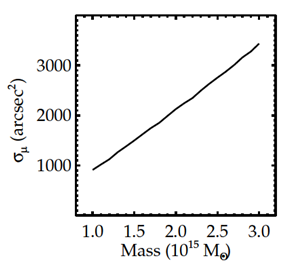
\includegraphics[width=0.4\textwidth]{../Images/Lensing_cross_section_as_a_function_of_mass.png}
			\caption[Lensing cross section as a function of mass]{\cite{Optimal_mass_configurations}Plot of the lensing cross section as a function of mass for a spherical halo at $z=0.5$. The dependence of cross section on mass can be clearly seen, indicating that the more massive a cluster, the better a lens it will be.\label{fig:Lensing_cross_section_as_a_function_of_mass}}
		\end{figure}

		The redshift of the lens must also be tightly constrained since the magnification depends on this. There is a balance to be struck when choosing the lens redshift for the strategy. On the one hand, the Einstein angle, an indicator of the strength of a lens, increases as the lens redshift decreases. Figure~\ref{fig:Einstein_angle_as_a_function_of_source_redshift} shows how lens redshift varies with Einstein angle. The point at which each curve crosses the x-axis is the lens redshift since no lensing occurs when the source and lens redshifts are equal. For each lens redshift, the Einstein angle increases rapidly for source redshifts slightly greater than that of the lens, and then quickly saturates. \cite{Constraining_source_redshift_distributions}
		\begin{figure}[!htbp]
			\centering
				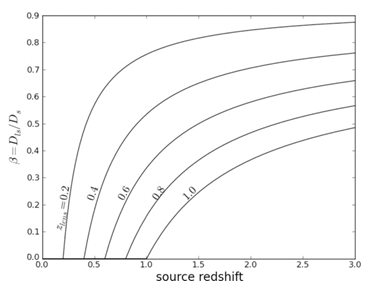
\includegraphics[width=0.5\textwidth]{../Images/Einstein_angle_as_a_function_of_source_redshift.png}
			\caption[Einstein angle as a function of source redshift]{\cite{Constraining_source_redshift_distributions} Plot of Einstein angle against source redshift. Again, each line corresponds to a different lens redshift. The point at which each line crosses the x-axis is the lens redshift, since at the lens, the magnification of the source is equal to 0.\label{fig:Einstein_angle_as_a_function_of_source_redshift}}
		\end{figure}

		However, the extent to which the images are distorted is not taken into account. The shear caused by a lens at a particular redshift is given by
		\begin{align}
			\gamma(r) &= \frac{4\pi G}{c^2}\frac{D_{LS}D_L}{D_S}\left( \overline{\Sigma}(<r)-\Sigma(r) \right)
		\end{align}
		where $\overline{\Sigma}(<r)$ is the mean projected surface mass density within r and $\Sigma(r)$ the projected surface mass density at $r$. Keeping the radius (and therefore surface mass density) constant, Figure~\ref{fig:shear_as_a_function_of_source_redshift} shows the dependence of shear on source redshift at fixed lens redshifts as the plot above. lens redshifts as the plot above. It can be seen from this plot, that at low source redshifts, the shear distortion is immeasurably small. As the redshift increases to around 0.5, the clusters at the lowest redshifts cause some significant distortion. Once the source redshift is greater than 1, shear distortion is seen around clusters at all the lens redshifts plotted\cite{Constraining_source_redshift_distributions}.
		\begin{figure}[!htbp]
			\centering
				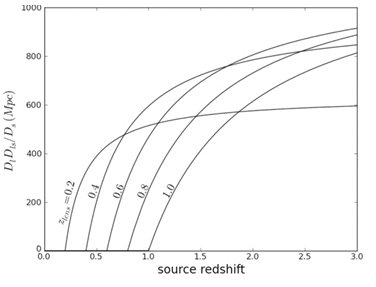
\includegraphics[width=0.5\textwidth]{../Images/Shear_as_a_function_of_source_redshift.png}
			\caption[Shear as a function of source redshift]{\cite{Constraining_source_redshift_distributions}A plot of shear against source redshift, with each line representing a different lens redshift. The point at which the lines cross the x-axis is the lens redshift, since at the lens, the magnification of the source is equal to 0.\label{fig:shear_as_a_function_of_source_redshift}}
		\end{figure}

		It has also been found that giant arcs are most likely to form behind higher redshift lenses, as shown in figure[arc probability]. Giant arcs are observed in systems where the shear is large. Lensing clusters at a redshift above 0.5 have been found to have an arc formation probability up to 3 times that of lower redshift lenses. The clusters observed at z>0.5 were also found to be generally less massive than closer clusters, indicating that clusters at this redshift are more efficient lenses. As a result, a judicious choice of lens redshift must be made to optimise both lensing strength and distortion for the best chance of observing high redshift galaxies. \cite{ wu_and_chiueh }
		\begin{figure}[!htbp]
			\centering
				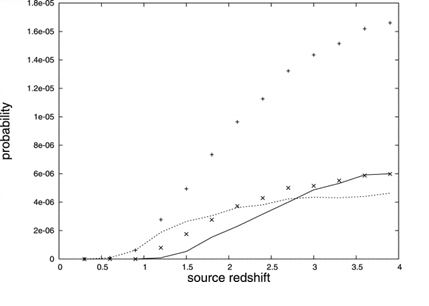
\includegraphics[width=0.5\textwidth]{../Images/Arc_probability.png}
			\caption[Arc probability]{\cite{wu_and_chiueh}Plot of the arc probability against source redshifts in four different lens intervals, $0.14\le z_L\le 0.45$ (dotted line), $0.49\le z_L\le 0.68$ (crosses), $0.73\le z_L\le 0.94$ (solid line), and $0.14\le z_L\le 0.94$ (plus signs).\label{fig:shear_as_a_function_of_source_redshift}}
		\end{figure}
	% subsection constraints_on_the_lenses (end)

	\subsection{Locating New Lenses} % (fold)
	\label{sub:locating_new_lenses}
		Locating new lenses would be advantageous in that the lenses could be chosen with the tight constraints specified above such that their properties are tailored to suit the needs of our strategy. The lenses would be selected using some form of wide survey by means of their strong lensing properties since objects that lense strongly are likely to be better for observing very faint sources. Taking the Einstein radius to be the average distance of the arcs from the centre of the lens, and assuming that most of the mass of the cluster is enclosed within this radius, an estimate of the mass can be found from
		\begin{align}
			M &= \Sigma_c\pi \theta_E^2 \label{eq:new_lens_mass_estimate}
		\end{align}
		The critical surface density, as defined in Equation~\ref{eq:new_lens_mass_estimate} can be found when the source redshift is known and the magnification of the source can then be calculated as detailed in section gravitational lensing results.
	% subsection locating_new_lenses (end)

	\subsection{Using Known Lenses} % (fold)
	\label{sub:using_known_lenses}
		The second option, selecting known lenses has the advantage that the masses and velocity dispersions would already be well determined, allowing an accurate calculation of the magnification to be made. Examples of surveys that have been carried out previously include Cluster Lens And Supernova survey with Hubble (CLASH)\cite{CLASH} and the MAssive Cluster Survey (MACS)\cite{MACS}. There are only a limited number of massive clusters known, however even with the small sample available, many interesting sources have already been observed for example a candidate $z\approx11$ galaxy behind cluster MACSJ0647.7+7015\cite{CLASH_z11_candidate}. Unless a wide survey is carried out as part of the observing strategy, using known lenses would significantly reduce the observing time required for the strategy compared to requiring an additional survey to locate new lenses. Both MACS and CLASH select their source using x-rays in order to obtain an unbiased distribution of masses, however, for this strategy the lenses will be chosen based on their masses and lensing properties.

		\subsubsection{Calculations on Magnification} % (fold)
		\label{ssub:calculations_on_magnification}
			The following calculations were carried out in order to quantify the number of extra objects one would expect to see with a lens. A magnification factor $\mu$ is chosen, for example 10. This corresponds to a change in AB magnitude given by
			\begin{align}
				AB_\text{change} &= -2.5\log_{10}(\mu)
			\end{align}
			which yields $-2.5$ for a magnification of 10. The fraction of the Einstein radius within which a source will be magnified by at least the value of $\mu$ is given to good approximation by\cite{Lens_mass_estimate}
			\begin{align}
				x_E &= \frac{\mu}{\mu -1}
			\end{align}
			Using the velocity dispersion of the cluster $\sigma$ and the angular diameter distances to the lens $D_L$ and source $D_S$ respectively, the following expression is also found to yield the Einstein angle,
			\begin{align}
				\theta_E &= \frac{4\pi G}{c^2}\frac{D_S-D_L}{D_S}
			\end{align}
			Using the Einstein angle in units of arcseconds, the area in degrees within which a certain magnification is exceeded is given by
			\begin{align}
				A &= \frac{\pi(x_E \theta_E)^2}{3600^2}
			\end{align}
			This area is calculated for source redshifts 1--15 and lens redshifts 0.1--1. Using results from the programme written by the predictions subgroup which gives a value for the number of galaxies per square degree, the area calculated above is multiplied by each value, giving a number of sources magnified at each redshift and magnitude. If the area, $A$, is found to be larger than the field of view of the telescope being used, the field of view of the telescope used as the value of $A$, since objects magnified outside of the field of view will not be observed. To find the number of extra galaxies seen with a lens between certain redshifts, one can sum the sources magnified enough to be seen in the redshift range of interest. For example, for a magnification of 10, sources as dim as magnitude 34.1 can be seen with JWST (without the lens, JWST would be limited to magnitude 31.6). One would sum for example redshifts 10-12 for magnitudes 31.6-34.1 to find the additional number of galaxies seen in this range.

			The magnification factors considered for these calculations are 15, 10, 5, 2.5 and 1.5 which enable telescopes to see magnitudes of 2.94, 2.5, 1.75, 1 and 0.44 deeper respectively. Selecting a lens at a redshift of 0.6 as an example, table~\ref{tab:areas_table} shows the area magnified by a given factor for a range of source redshifts.
			\begin{table}[!htbp]
				\begin{center}
					\begin{tabular}{c|c|c|c|c|c}
						Source $z$ 	&$\mu=1.5$	&$\mu=2.5$	&$\mu=5$	&$\mu=10$	&$\mu=15$ \\
						\hline \hline
					10	&\num{1.08e-3} 	&\num{3.33e-4} 	&\num{1.87e-4} 	&\num{1.48e-4} 	&\num{1.38e-4} \\
					11	&\num{1.09e-3} 	&\num{3.37e-4} 	&\num{1.90e-4} 	&\num{1.50e-4} 	&\num{1.39e-4} \\
					12	&\num{1.10e-3} 	&\num{3.41e-4} 	&\num{1.92e-4} 	&\num{1.51e-4} 	&\num{1.41e-4} \\
					13	&\num{1.11e-3} 	&\num{3.44e-4} 	&\num{1.93e-4} 	&\num{1.53e-4} 	&\num{1.42e-4} \\
					14	&\num{1.12e-3} 	&\num{3.46e-4} 	&\num{1.95e-4} 	&\num{1.54e-4} 	&\num{1.43e-4} \\
					15	&\num{1.13e-3} 	&\num{3.49e-4} 	&\num{1.96e-4} 	&\num{1.55e-4} 	&\num{1.44e-4}
					\end{tabular}
				\end{center}
				\caption[areas table]{Area within which the magnification factor is greater than certain values. These areas have been calculated using a lens redshift of 0.6 and a velocity dispersion of \SI{1000}{\kilo\metre\per\second}.\label{tab:areas_table}}
			\end{table}

			These areas correspond to the following numbers of extra sources observed at redshifts 10--15 for a cluster with velocity dispersion \SI{1000}{\kilo\metre\per\second} including any source now magnitude 31.6 or brighter.
			\begin{table}[!htbp]
				\begin{center}
					\begin{tabular}{c|c|c|c|c|c}
						Source $z$ 	&$1.5>\mu$	&$1.5>\mu>2.5$	&$10>\mu>5$	&$15>\mu>10$	&$\mu>15$ \\
						\hline \hline
						10--12 		&4.19 		&2.97 			&2.33 		&1.42 			&25.2 \\
						12--15 		&1.21 		&1.04 			&1.00 		&0.70 			&13.2
					\end{tabular}
				\end{center}
				\caption[source numbers table]{Number of objects magnified by each factor, calculated from the areas in table~\ref{tab:areas_table} and the predictions group's program.\label{tab:source_numbers_table}}
			\end{table}

			From Table~\ref{tab:source_numbers_table}, the number of sources observed that have been magnified by a factor greater than 15 is the highest. This is unsurprising, since at greater magnifications, the deepest sources will be observed, and the number density of galaxies is predicted to increase rapidly at dimmer magnitudes. Furthermore, the area within this smallest circle is larger than the differences between the intermediate areas. Once the magnification is as low as 2.5, however, the number begins to increase again, since the area within which such small magnifications can occur become very large. Figures~\ref{distribution_of_magnification1} and \ref{distribution_of_magnification2} show the distribution of redshifts of the magnified objects.
			% \begin{figure}[!htbp]
			% 	\centering
			% 		\begingroup\endlinechar=-1
			% 			\resizebox{0.8\textwidth}{!}{%
			% 				% GNUPLOT: LaTeX picture with Postscript
\begingroup
  \makeatletter
  \providecommand\color[2][]{%
    \GenericError{(gnuplot) \space\space\space\@spaces}{%
      Package color not loaded in conjunction with
      terminal option `colourtext'%
    }{See the gnuplot documentation for explanation.%
    }{Either use 'blacktext' in gnuplot or load the package
      color.sty in LaTeX.}%
    \renewcommand\color[2][]{}%
  }%
  \providecommand\includegraphics[2][]{%
    \GenericError{(gnuplot) \space\space\space\@spaces}{%
      Package graphicx or graphics not loaded%
    }{See the gnuplot documentation for explanation.%
    }{The gnuplot epslatex terminal needs graphicx.sty or graphics.sty.}%
    \renewcommand\includegraphics[2][]{}%
  }%
  \providecommand\rotatebox[2]{#2}%
  \@ifundefined{ifGPcolor}{%
    \newif\ifGPcolor
    \GPcolortrue
  }{}%
  \@ifundefined{ifGPblacktext}{%
    \newif\ifGPblacktext
    \GPblacktexttrue
  }{}%
  % define a \g@addto@macro without @ in the name:
  \let\gplgaddtomacro\g@addto@macro
  % define empty templates for all commands taking text:
  \gdef\gplbacktext{}%
  \gdef\gplfronttext{}%
  \makeatother
  \ifGPblacktext
    % no textcolor at all
    \def\colorrgb#1{}%
    \def\colorgray#1{}%
  \else
    % gray or color?
    \ifGPcolor
      \def\colorrgb#1{\color[rgb]{#1}}%
      \def\colorgray#1{\color[gray]{#1}}%
      \expandafter\def\csname LTw\endcsname{\color{white}}%
      \expandafter\def\csname LTb\endcsname{\color{black}}%
      \expandafter\def\csname LTa\endcsname{\color{black}}%
      \expandafter\def\csname LT0\endcsname{\color[rgb]{1,0,0}}%
      \expandafter\def\csname LT1\endcsname{\color[rgb]{0,1,0}}%
      \expandafter\def\csname LT2\endcsname{\color[rgb]{0,0,1}}%
      \expandafter\def\csname LT3\endcsname{\color[rgb]{1,0,1}}%
      \expandafter\def\csname LT4\endcsname{\color[rgb]{0,1,1}}%
      \expandafter\def\csname LT5\endcsname{\color[rgb]{1,1,0}}%
      \expandafter\def\csname LT6\endcsname{\color[rgb]{0,0,0}}%
      \expandafter\def\csname LT7\endcsname{\color[rgb]{1,0.3,0}}%
      \expandafter\def\csname LT8\endcsname{\color[rgb]{0.5,0.5,0.5}}%
    \else
      % gray
      \def\colorrgb#1{\color{black}}%
      \def\colorgray#1{\color[gray]{#1}}%
      \expandafter\def\csname LTw\endcsname{\color{white}}%
      \expandafter\def\csname LTb\endcsname{\color{black}}%
      \expandafter\def\csname LTa\endcsname{\color{black}}%
      \expandafter\def\csname LT0\endcsname{\color{black}}%
      \expandafter\def\csname LT1\endcsname{\color{black}}%
      \expandafter\def\csname LT2\endcsname{\color{black}}%
      \expandafter\def\csname LT3\endcsname{\color{black}}%
      \expandafter\def\csname LT4\endcsname{\color{black}}%
      \expandafter\def\csname LT5\endcsname{\color{black}}%
      \expandafter\def\csname LT6\endcsname{\color{black}}%
      \expandafter\def\csname LT7\endcsname{\color{black}}%
      \expandafter\def\csname LT8\endcsname{\color{black}}%
    \fi
  \fi
  \setlength{\unitlength}{0.0500bp}%
  \begin{picture}(7200.00,4320.00)%
    \gplgaddtomacro\gplbacktext{%
      \put(543,595){\makebox(0,0)[r]{\strut{} 0}}%
      \put(543,986){\makebox(0,0)[r]{\strut{} 1}}%
      \put(543,1377){\makebox(0,0)[r]{\strut{} 2}}%
      \put(543,1768){\makebox(0,0)[r]{\strut{} 3}}%
      \put(543,2159){\makebox(0,0)[r]{\strut{} 4}}%
      \put(543,2551){\makebox(0,0)[r]{\strut{} 5}}%
      \put(543,2942){\makebox(0,0)[r]{\strut{} 6}}%
      \put(543,3333){\makebox(0,0)[r]{\strut{} 7}}%
      \put(543,3724){\makebox(0,0)[r]{\strut{} 8}}%
      \put(543,4115){\makebox(0,0)[r]{\strut{} 9}}%
      \put(1213,409){\makebox(0,0){\strut{} 10}}%
      \put(2349,409){\makebox(0,0){\strut{} 11}}%
      \put(3485,409){\makebox(0,0){\strut{} 12}}%
      \put(4621,409){\makebox(0,0){\strut{} 13}}%
      \put(5757,409){\makebox(0,0){\strut{} 14}}%
      \put(6893,409){\makebox(0,0){\strut{} 15}}%
      \csname LTb\endcsname%
      \put(144,2355){\rotatebox{-270}{\makebox(0,0){\strut{}Number of Galaxies}}}%
      \csname LTb\endcsname%
      \put(3769,130){\makebox(0,0){\strut{}Magnitude ($M$)}}%
      \put(3769,4022){\makebox(0,0){\strut{}}}%
    }%
    \gplgaddtomacro\gplfronttext{%
      \csname LTb\endcsname%
      \put(5980,3631){\makebox(0,0)[r]{\strut{}\SI{0.1e6}{\second}}}%
      \csname LTb\endcsname%
      \put(5980,3445){\makebox(0,0)[r]{\strut{}\SI{0.2e6}{\second}}}%
      \csname LTb\endcsname%
      \put(5980,3259){\makebox(0,0)[r]{\strut{}\SI{0.5e6}{\second}}}%
      \csname LTb\endcsname%
      \put(5980,3073){\makebox(0,0)[r]{\strut{}\SI{0.5e6}{\second}}}%
      \csname LTb\endcsname%
      \put(5980,2887){\makebox(0,0)[r]{\strut{}\SI{0.5e6}{\second}}}%
    }%
    \gplbacktext
    \put(0,0){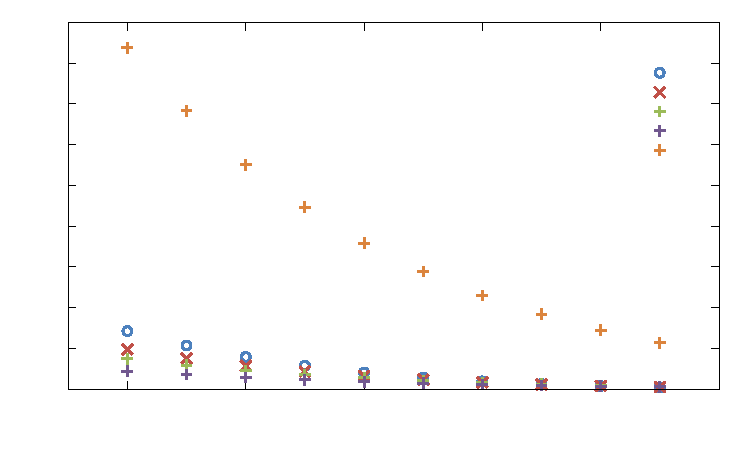
\includegraphics{GRAPH_distribution_of_magnification1}}%
    \gplfronttext
  \end{picture}%
\endgroup

			% 			}\endgroup
			% 	\caption{Number of galaxies expected for different magnitudes, given set overall observing time (JW 6--8.5).\label{fig:galaxies_expected_JWST_6-8}}
			% \end{figure}
			\begin{figure}[!htbp]
	        	\begin{minipage}[c]{0.5\linewidth}
					\centering
						\begingroup\endlinechar=-1
							\resizebox{0.9\textwidth}{!}{%
								% GNUPLOT: LaTeX picture with Postscript
\begingroup
  \makeatletter
  \providecommand\color[2][]{%
    \GenericError{(gnuplot) \space\space\space\@spaces}{%
      Package color not loaded in conjunction with
      terminal option `colourtext'%
    }{See the gnuplot documentation for explanation.%
    }{Either use 'blacktext' in gnuplot or load the package
      color.sty in LaTeX.}%
    \renewcommand\color[2][]{}%
  }%
  \providecommand\includegraphics[2][]{%
    \GenericError{(gnuplot) \space\space\space\@spaces}{%
      Package graphicx or graphics not loaded%
    }{See the gnuplot documentation for explanation.%
    }{The gnuplot epslatex terminal needs graphicx.sty or graphics.sty.}%
    \renewcommand\includegraphics[2][]{}%
  }%
  \providecommand\rotatebox[2]{#2}%
  \@ifundefined{ifGPcolor}{%
    \newif\ifGPcolor
    \GPcolortrue
  }{}%
  \@ifundefined{ifGPblacktext}{%
    \newif\ifGPblacktext
    \GPblacktexttrue
  }{}%
  % define a \g@addto@macro without @ in the name:
  \let\gplgaddtomacro\g@addto@macro
  % define empty templates for all commands taking text:
  \gdef\gplbacktext{}%
  \gdef\gplfronttext{}%
  \makeatother
  \ifGPblacktext
    % no textcolor at all
    \def\colorrgb#1{}%
    \def\colorgray#1{}%
  \else
    % gray or color?
    \ifGPcolor
      \def\colorrgb#1{\color[rgb]{#1}}%
      \def\colorgray#1{\color[gray]{#1}}%
      \expandafter\def\csname LTw\endcsname{\color{white}}%
      \expandafter\def\csname LTb\endcsname{\color{black}}%
      \expandafter\def\csname LTa\endcsname{\color{black}}%
      \expandafter\def\csname LT0\endcsname{\color[rgb]{1,0,0}}%
      \expandafter\def\csname LT1\endcsname{\color[rgb]{0,1,0}}%
      \expandafter\def\csname LT2\endcsname{\color[rgb]{0,0,1}}%
      \expandafter\def\csname LT3\endcsname{\color[rgb]{1,0,1}}%
      \expandafter\def\csname LT4\endcsname{\color[rgb]{0,1,1}}%
      \expandafter\def\csname LT5\endcsname{\color[rgb]{1,1,0}}%
      \expandafter\def\csname LT6\endcsname{\color[rgb]{0,0,0}}%
      \expandafter\def\csname LT7\endcsname{\color[rgb]{1,0.3,0}}%
      \expandafter\def\csname LT8\endcsname{\color[rgb]{0.5,0.5,0.5}}%
    \else
      % gray
      \def\colorrgb#1{\color{black}}%
      \def\colorgray#1{\color[gray]{#1}}%
      \expandafter\def\csname LTw\endcsname{\color{white}}%
      \expandafter\def\csname LTb\endcsname{\color{black}}%
      \expandafter\def\csname LTa\endcsname{\color{black}}%
      \expandafter\def\csname LT0\endcsname{\color{black}}%
      \expandafter\def\csname LT1\endcsname{\color{black}}%
      \expandafter\def\csname LT2\endcsname{\color{black}}%
      \expandafter\def\csname LT3\endcsname{\color{black}}%
      \expandafter\def\csname LT4\endcsname{\color{black}}%
      \expandafter\def\csname LT5\endcsname{\color{black}}%
      \expandafter\def\csname LT6\endcsname{\color{black}}%
      \expandafter\def\csname LT7\endcsname{\color{black}}%
      \expandafter\def\csname LT8\endcsname{\color{black}}%
    \fi
  \fi
  \setlength{\unitlength}{0.0500bp}%
  \begin{picture}(7200.00,4320.00)%
    \gplgaddtomacro\gplbacktext{%
      \put(543,595){\makebox(0,0)[r]{\strut{} 0}}%
      \put(543,986){\makebox(0,0)[r]{\strut{} 1}}%
      \put(543,1377){\makebox(0,0)[r]{\strut{} 2}}%
      \put(543,1768){\makebox(0,0)[r]{\strut{} 3}}%
      \put(543,2159){\makebox(0,0)[r]{\strut{} 4}}%
      \put(543,2551){\makebox(0,0)[r]{\strut{} 5}}%
      \put(543,2942){\makebox(0,0)[r]{\strut{} 6}}%
      \put(543,3333){\makebox(0,0)[r]{\strut{} 7}}%
      \put(543,3724){\makebox(0,0)[r]{\strut{} 8}}%
      \put(543,4115){\makebox(0,0)[r]{\strut{} 9}}%
      \put(1213,409){\makebox(0,0){\strut{} 10}}%
      \put(2349,409){\makebox(0,0){\strut{} 11}}%
      \put(3485,409){\makebox(0,0){\strut{} 12}}%
      \put(4621,409){\makebox(0,0){\strut{} 13}}%
      \put(5757,409){\makebox(0,0){\strut{} 14}}%
      \put(6893,409){\makebox(0,0){\strut{} 15}}%
      \csname LTb\endcsname%
      \put(144,2355){\rotatebox{-270}{\makebox(0,0){\strut{}Number of Galaxies}}}%
      \csname LTb\endcsname%
      \put(3769,130){\makebox(0,0){\strut{}Magnitude ($M$)}}%
      \put(3769,4022){\makebox(0,0){\strut{}}}%
    }%
    \gplgaddtomacro\gplfronttext{%
      \csname LTb\endcsname%
      \put(5980,3631){\makebox(0,0)[r]{\strut{}\SI{0.1e6}{\second}}}%
      \csname LTb\endcsname%
      \put(5980,3445){\makebox(0,0)[r]{\strut{}\SI{0.2e6}{\second}}}%
      \csname LTb\endcsname%
      \put(5980,3259){\makebox(0,0)[r]{\strut{}\SI{0.5e6}{\second}}}%
      \csname LTb\endcsname%
      \put(5980,3073){\makebox(0,0)[r]{\strut{}\SI{0.5e6}{\second}}}%
      \csname LTb\endcsname%
      \put(5980,2887){\makebox(0,0)[r]{\strut{}\SI{0.5e6}{\second}}}%
    }%
    \gplbacktext
    \put(0,0){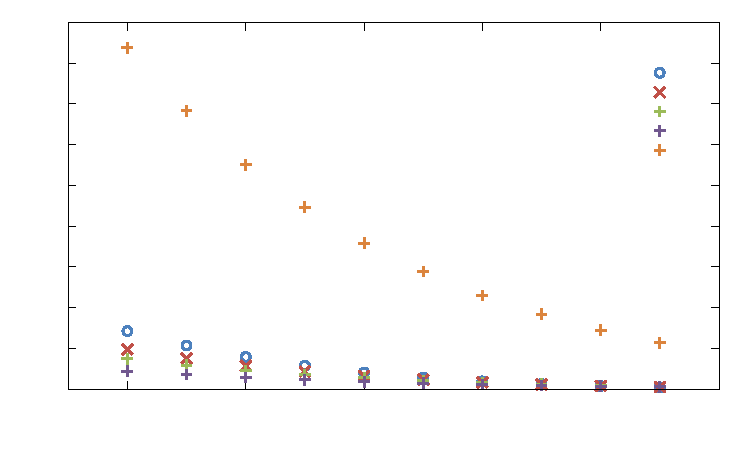
\includegraphics{GRAPH_distribution_of_magnification1}}%
    \gplfronttext
  \end{picture}%
\endgroup

							}\endgroup
					\caption{Number of galaxies expected for different magnitudes, given set overall observing time (E-ELT 6--8.5).\label{fig:distribution_of_magnification1}}
				\end{minipage}
	        	\begin{minipage}[c]{0.5\linewidth}
					\centering
						\begingroup\endlinechar=-1
							\resizebox{0.9\textwidth}{!}{%
								% GNUPLOT: LaTeX picture with Postscript
\begingroup
  \makeatletter
  \providecommand\color[2][]{%
    \GenericError{(gnuplot) \space\space\space\@spaces}{%
      Package color not loaded in conjunction with
      terminal option `colourtext'%
    }{See the gnuplot documentation for explanation.%
    }{Either use 'blacktext' in gnuplot or load the package
      color.sty in LaTeX.}%
    \renewcommand\color[2][]{}%
  }%
  \providecommand\includegraphics[2][]{%
    \GenericError{(gnuplot) \space\space\space\@spaces}{%
      Package graphicx or graphics not loaded%
    }{See the gnuplot documentation for explanation.%
    }{The gnuplot epslatex terminal needs graphicx.sty or graphics.sty.}%
    \renewcommand\includegraphics[2][]{}%
  }%
  \providecommand\rotatebox[2]{#2}%
  \@ifundefined{ifGPcolor}{%
    \newif\ifGPcolor
    \GPcolortrue
  }{}%
  \@ifundefined{ifGPblacktext}{%
    \newif\ifGPblacktext
    \GPblacktexttrue
  }{}%
  % define a \g@addto@macro without @ in the name:
  \let\gplgaddtomacro\g@addto@macro
  % define empty templates for all commands taking text:
  \gdef\gplbacktext{}%
  \gdef\gplfronttext{}%
  \makeatother
  \ifGPblacktext
    % no textcolor at all
    \def\colorrgb#1{}%
    \def\colorgray#1{}%
  \else
    % gray or color?
    \ifGPcolor
      \def\colorrgb#1{\color[rgb]{#1}}%
      \def\colorgray#1{\color[gray]{#1}}%
      \expandafter\def\csname LTw\endcsname{\color{white}}%
      \expandafter\def\csname LTb\endcsname{\color{black}}%
      \expandafter\def\csname LTa\endcsname{\color{black}}%
      \expandafter\def\csname LT0\endcsname{\color[rgb]{1,0,0}}%
      \expandafter\def\csname LT1\endcsname{\color[rgb]{0,1,0}}%
      \expandafter\def\csname LT2\endcsname{\color[rgb]{0,0,1}}%
      \expandafter\def\csname LT3\endcsname{\color[rgb]{1,0,1}}%
      \expandafter\def\csname LT4\endcsname{\color[rgb]{0,1,1}}%
      \expandafter\def\csname LT5\endcsname{\color[rgb]{1,1,0}}%
      \expandafter\def\csname LT6\endcsname{\color[rgb]{0,0,0}}%
      \expandafter\def\csname LT7\endcsname{\color[rgb]{1,0.3,0}}%
      \expandafter\def\csname LT8\endcsname{\color[rgb]{0.5,0.5,0.5}}%
    \else
      % gray
      \def\colorrgb#1{\color{black}}%
      \def\colorgray#1{\color[gray]{#1}}%
      \expandafter\def\csname LTw\endcsname{\color{white}}%
      \expandafter\def\csname LTb\endcsname{\color{black}}%
      \expandafter\def\csname LTa\endcsname{\color{black}}%
      \expandafter\def\csname LT0\endcsname{\color{black}}%
      \expandafter\def\csname LT1\endcsname{\color{black}}%
      \expandafter\def\csname LT2\endcsname{\color{black}}%
      \expandafter\def\csname LT3\endcsname{\color{black}}%
      \expandafter\def\csname LT4\endcsname{\color{black}}%
      \expandafter\def\csname LT5\endcsname{\color{black}}%
      \expandafter\def\csname LT6\endcsname{\color{black}}%
      \expandafter\def\csname LT7\endcsname{\color{black}}%
      \expandafter\def\csname LT8\endcsname{\color{black}}%
    \fi
  \fi
  \setlength{\unitlength}{0.0500bp}%
  \begin{picture}(7200.00,4320.00)%
    \gplgaddtomacro\gplbacktext{%
      \put(747,595){\makebox(0,0)[r]{\strut{} 0}}%
      \put(747,1035){\makebox(0,0)[r]{\strut{} 0.2}}%
      \put(747,1475){\makebox(0,0)[r]{\strut{} 0.4}}%
      \put(747,1915){\makebox(0,0)[r]{\strut{} 0.6}}%
      \put(747,2355){\makebox(0,0)[r]{\strut{} 0.8}}%
      \put(747,2795){\makebox(0,0)[r]{\strut{} 1}}%
      \put(747,3235){\makebox(0,0)[r]{\strut{} 1.2}}%
      \put(747,3675){\makebox(0,0)[r]{\strut{} 1.4}}%
      \put(747,4115){\makebox(0,0)[r]{\strut{} 1.6}}%
      \put(1398,409){\makebox(0,0){\strut{} 10}}%
      \put(2497,409){\makebox(0,0){\strut{} 11}}%
      \put(3596,409){\makebox(0,0){\strut{} 12}}%
      \put(4695,409){\makebox(0,0){\strut{} 13}}%
      \put(5794,409){\makebox(0,0){\strut{} 14}}%
      \put(6893,409){\makebox(0,0){\strut{} 15}}%
      \csname LTb\endcsname%
      \put(144,2355){\rotatebox{-270}{\makebox(0,0){\strut{}Number of Galaxies}}}%
      \csname LTb\endcsname%
      \put(3871,130){\makebox(0,0){\strut{}Magnitude ($M$)}}%
      \put(3871,4022){\makebox(0,0){\strut{}}}%
    }%
    \gplgaddtomacro\gplfronttext{%
      \csname LTb\endcsname%
      \put(5987,3802){\makebox(0,0)[r]{\strut{}\SI{0.1e6}{\second}}}%
      \csname LTb\endcsname%
      \put(5987,3616){\makebox(0,0)[r]{\strut{}\SI{0.2e6}{\second}}}%
      \csname LTb\endcsname%
      \put(5987,3430){\makebox(0,0)[r]{\strut{}\SI{0.5e6}{\second}}}%
      \csname LTb\endcsname%
      \put(5987,3244){\makebox(0,0)[r]{\strut{}\SI{0.5e6}{\second}}}%
    }%
    \gplbacktext
    \put(0,0){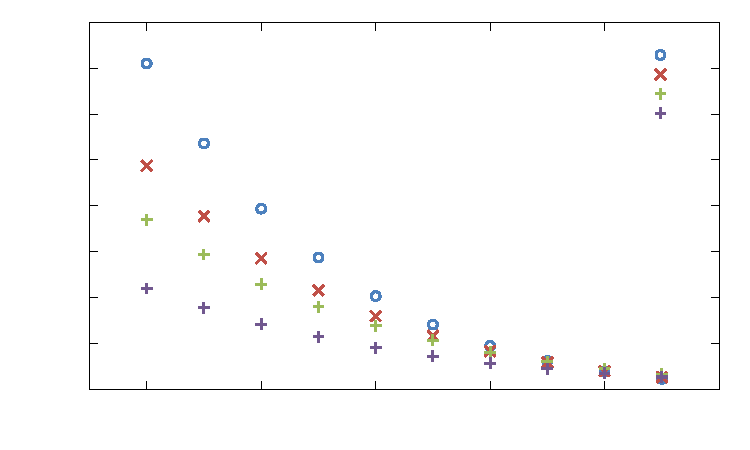
\includegraphics{GRAPH_distribution_of_magnification2}}%
    \gplfronttext
  \end{picture}%
\endgroup

							}\endgroup
					\caption{Number of galaxies expected for different magnitudes, given set overall observing time (E-ELT 6--8.5).\label{fig:distribution_of_magnification2}}
				\end{minipage}
			\end{figure}

			Even at the highest magnifications, few objects are expected at redshifts as high as 15, however at very small source angles, the magnification factor will be greater than 15 so there in the possibility of seeing very strongly lensed sources from even deeper redshifts.

			There is a trade-off when using gravitational lenses between the ability to see much deeper due to the magnification and the fact that the viewing area is decreased due to obscuration by the lens and the increased size of the images. The lower the redshift of the lenses chosen, the more significant this problem is, pushing the optimum lens redshift towards a higher value again. As a result, the most useful way to integrate gravitational lensing into the strategy is to use it as a supplement to the deep survey, to attempt to observe a few objects at extremely high redshift, rather than to magnify and better resolve sources that can be detected without a lens.
		% subsubsection calculations_on_magnification (end)
	% subsection using_known_lenses (end)
% section observational_gravitational_lensing (end)
